\documentclass[a4paper,10pt]{report}
\usepackage[utf8x]{inputenc}
\usepackage[T1]{fontenc}
\usepackage[french]{babel} 
\usepackage{lmodern} % Pour changer le pack de police
\usepackage{makeidx}
\usepackage{graphicx}
\graphicspath{{figures/}}
\usepackage[margin=3cm]{geometry}
\usepackage{array}
\usepackage{float}
\usepackage[cc]{titlepic}

\titlepic{
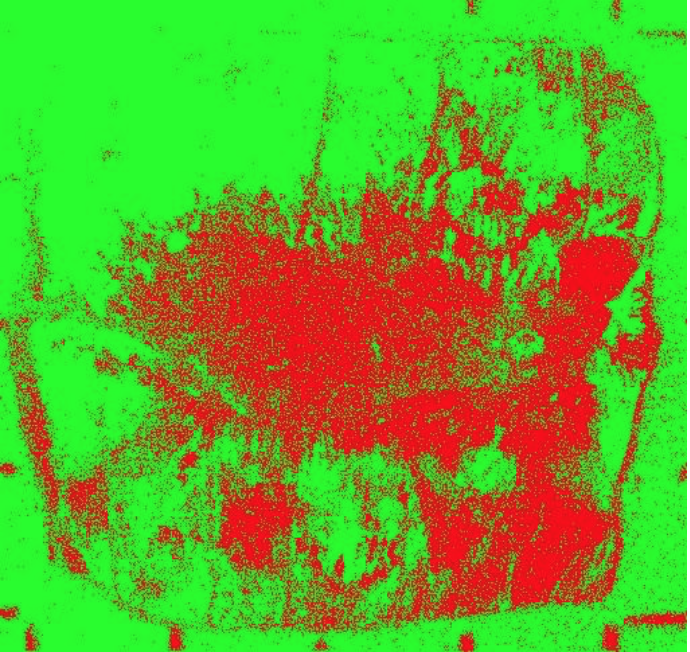
\includegraphics[width=7cm]{titlepic1.png}
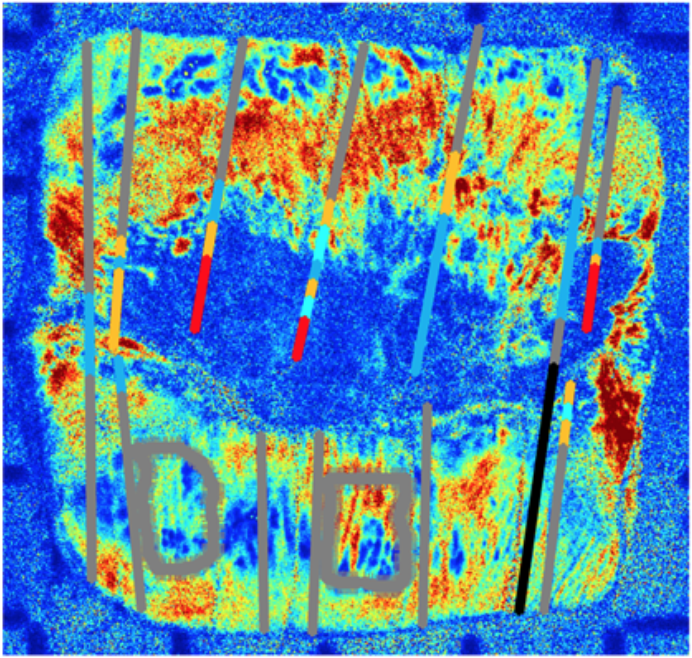
\includegraphics[width=7cm]{titlepic2.png}
}
\title{Projet 3A\\Analyse d'imagerie polarimétrique}
\author{\textsc{Guinaudeau} Alexandre\\
	\and 
	\textsc{Hulot} Pierre
	\and 
	\textsc{Dejoie} Etienne	
	}
\date{\today}
\makeindex 
\begin{document}

\maketitle

\begin{abstract}
Le résumé (abstract en anglais) de mon article.
\end{abstract}

\chapter{contexte}
\section{ADM Polar, contexte du projet}
Le principal partenaire du projet est ADM Polar est une start up d'imagerie médicale basée sur la collecte et l'analyse de données polarimétriques. L'objectif de la start up est d'utiliser ces données afin de diagnostiquer de façon automatisée un cancer (col de l'uterus). Une première étude in-vivo menée sur 140 patientes leur a fourni une large base de données sur laquelle ils comptent construire leur entreprise grâce à de l'analyse Big Data. Lors d'une événement du cabinet Start up, organisé par les élèves de l'école polytechnique (dont Étienne), nous les avons rencontré une première fois. Les membres de la start up sont alors venu vers nous en nous expliquant qu'ils avaient énormément de données à valoriser mais qu'ils ne savaient pas trop comment faire (leur domaine respectifs étant plutôt relié à la physique et au médical). Nous avons donc décider dans le cadre du projet 3A de nous lancer dans cette entreprise ambitieuse, à l'aide de nos connaissances en informatique et nos cours de Big Data. La start up étant localisée dans les laboratoires de l'école, cela a rendu plus simple les rencontre, les échanges et les suivis tout au long du projet.
\section{Présentation des données}
Pour ce projet nous disposions d'un jeu de données de $163 000$ pixels répartis sur 17 images différentes. Pour chaque pixel nous avions les 16 éléments de la matrice de Müller, leur position, leur diagnostic, et l'image correspondante.
Ces Pixels sont répartis en $4/5$ de sains et $1/5$ de malades. L'affichage des pixels nous montre que dans chaque image, les pixels sont répartis en zones au diagnostic identique. Sur les $17$ images, $11$ possèdent que des zones saines, une a une zone saine et une zone malade et les $5$ dernières ont que des zones malades. Le nombre d'images étant assez limité il n'a été facile de trouver des points communs aux pixels sain et aux pixels malades.

\begin{figure}[htbp]
  \caption{répartition des zones}
  \centering
  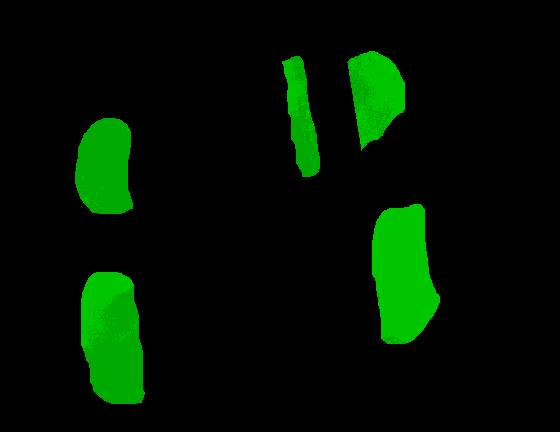
\includegraphics[width=3cm]{piece(1).jpg}
  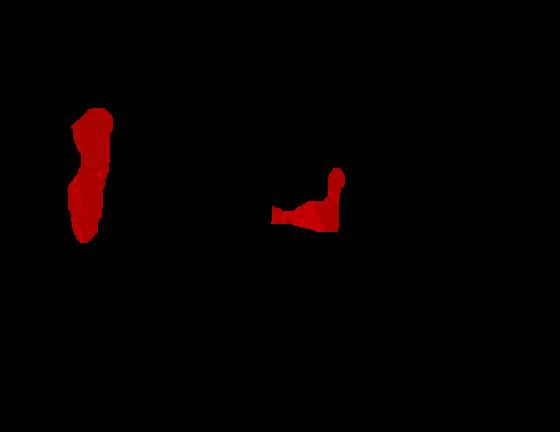
\includegraphics[width=3cm]{piece(2).jpg}
  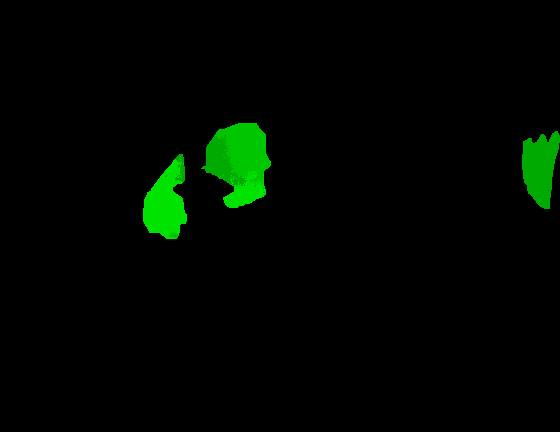
\includegraphics[width=3cm]{piece(3).jpg}
  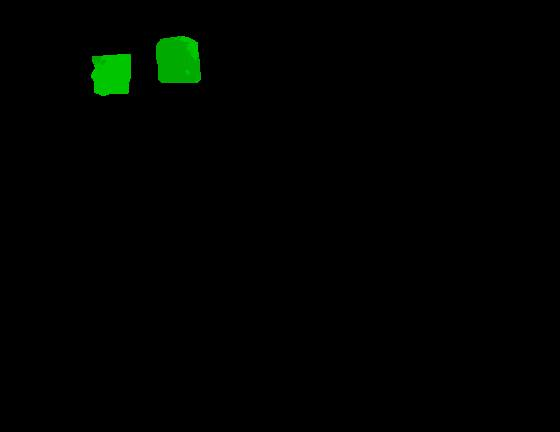
\includegraphics[width=3cm]{piece(4).jpg}
  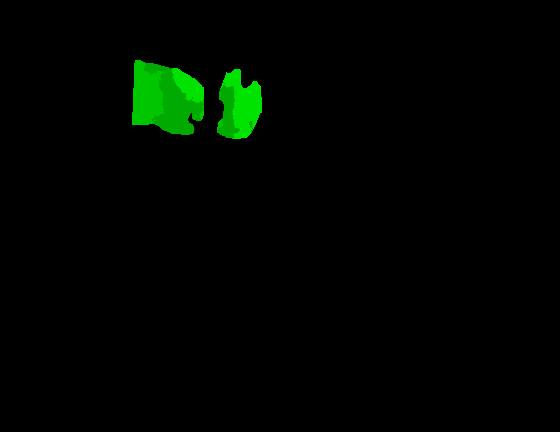
\includegraphics[width=3cm]{piece(5).jpg}
  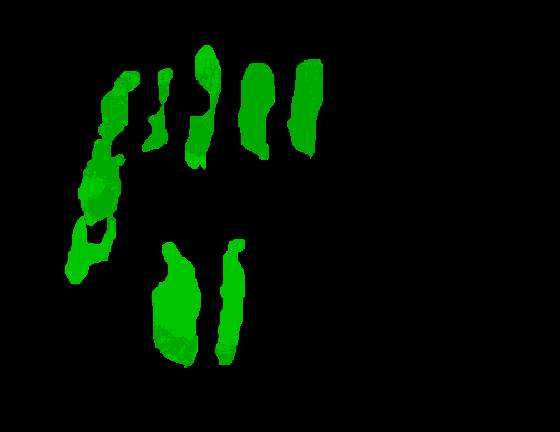
\includegraphics[width=3cm]{piece(6).jpg}
  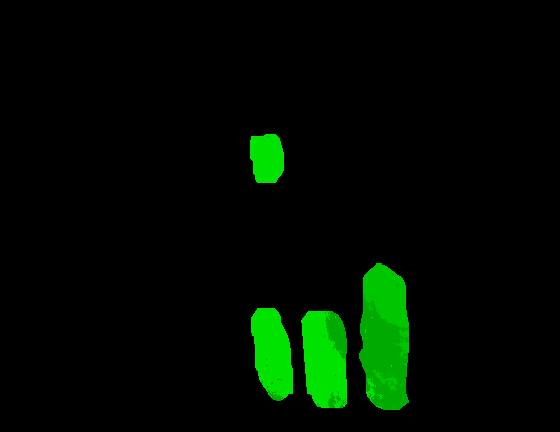
\includegraphics[width=3cm]{piece(7).jpg}
  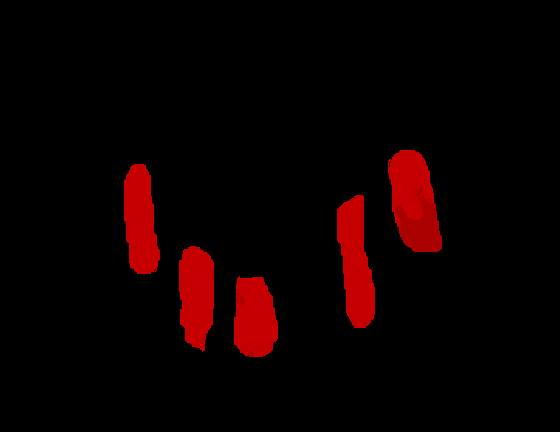
\includegraphics[width=3cm]{piece(8).jpg}
  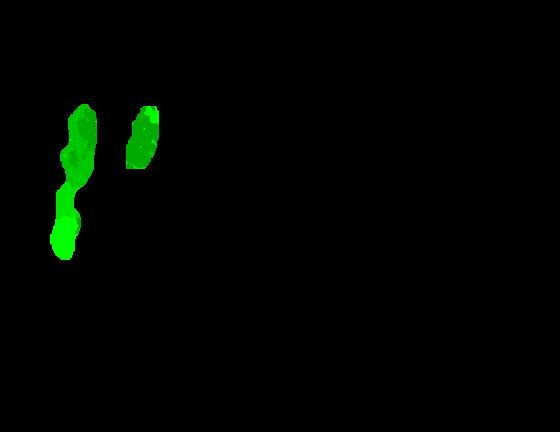
\includegraphics[width=3cm]{piece(9).jpg}
  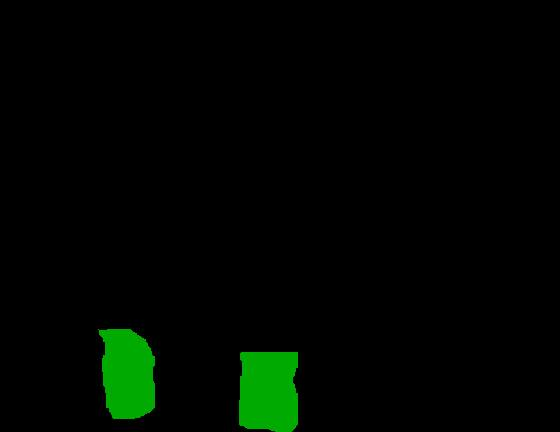
\includegraphics[width=3cm]{piece(10).jpg}
  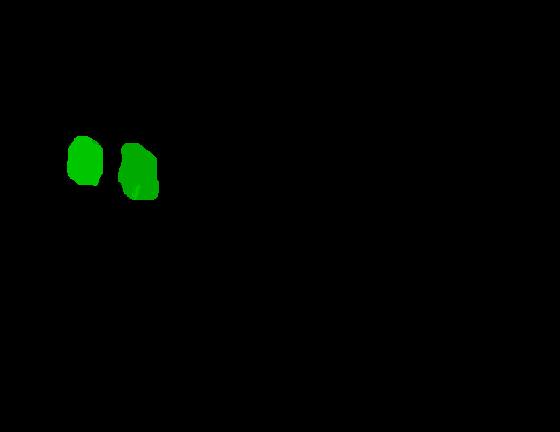
\includegraphics[width=3cm]{piece(11).jpg}
  
\includegraphics[width=3cm]{piece(12).jpg}
  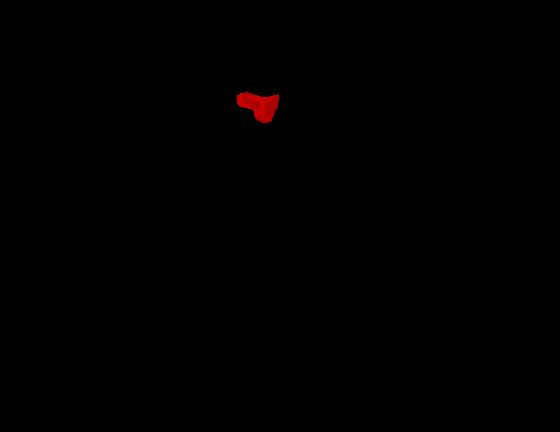
\includegraphics[width=3cm]{piece(13).jpg}
  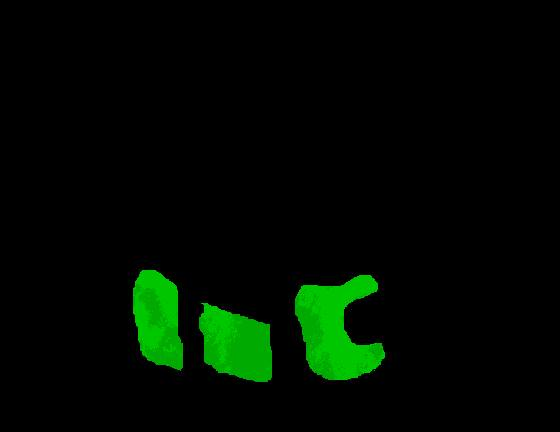
\includegraphics[width=3cm]{piece(14).jpg}
  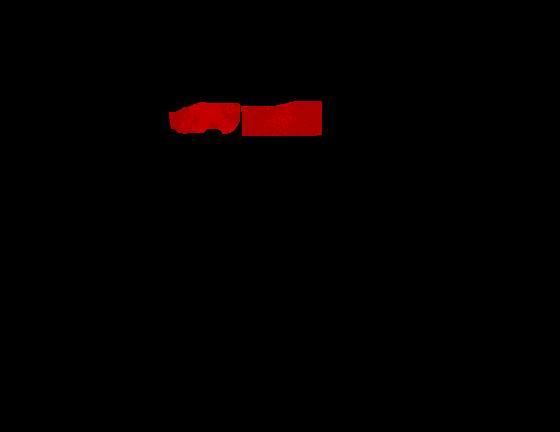
\includegraphics[width=3cm]{piece(15).jpg}
  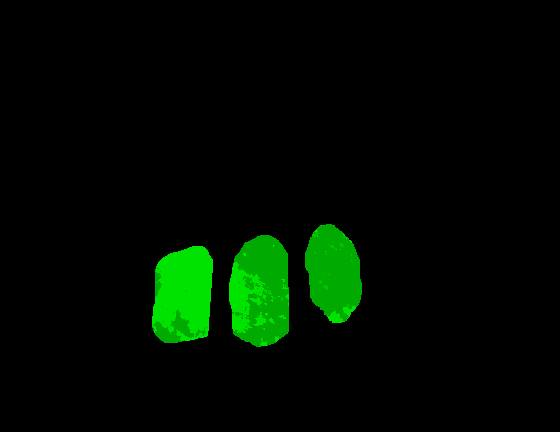
\includegraphics[width=3cm]{piece(16).jpg}
  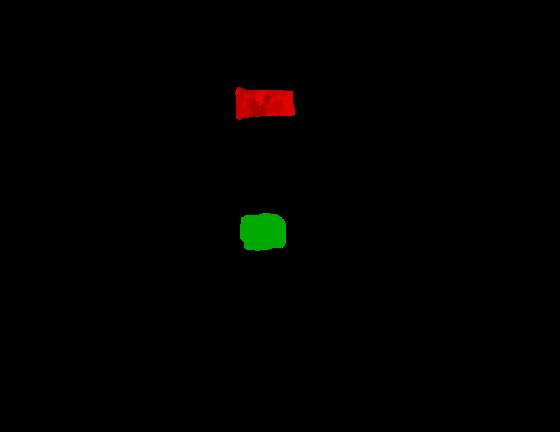
\includegraphics[width=3cm]{piece(17).jpg}
\end{figure}

\subsection{la Matrice de Müller}
\index{Matrice de Muller}
Les données sont obtenues par polarisation de la lumière. De la lumière polarisée est envoyée sur l'échantillon, réfléchi par celui ci est analysé ensuite.
La matrice de Müller est obtenue à partir de l'analyse de la polarisation de la lumière réfléchie. Le postulat du laboratoire sur lequel repose tout le traitement des données est que les cellules saines et malades polarisent différemment la lumière. Cela implique qu'il est possible de reconnaître une cellule malade par la polarisation de la lumière réfléchie.
Le PICM se bases pour cela d'observations de relation entre les images polarisées et le diagnostic. 
La polarisation génère 16 images par échantillon. On associe alors à chaque pixel une matrice $4x4$ appelée matrice de Müller. Dans cette matrice, la première ligne et la première colonne représentent l'intensité du signal, ces éléments influent peu sur le diagnostic mais ont des valeur élevés, ils introduisent beaucoup de biais et de sur-apprentissage. Nous avons donc décidé de ne pas les prendre en compte. Les éléments diagonaux sont normalement censé être les plus significatifs mais les reflets introduisent beaucoup de bruit rendant ces données difficilement utilisables. Il reste 6 éléments dans la matrices sur lesquels nous allons nous concentrer. 

\subsection{Le Clustering}
La disposition des données n'étant pas facilement exploitable directement il fallait réduire la complexité du problème, par exemple en limitant le nombre de données. Nous avons ainsi décidé de clustériser les données de chaque image afin d'en avoir beaucoup moins, mais plus significatives. La position du pixel dans l'image n'a pas été prise en compte, même si les zones résultantes sont proches. La clustérisation à été faite par un algorithme de type KNN (k plus proches voisins) sur les $6$ éléments significatifs de la matrice de Müller. Les diagnostics étant propres à chaque image (une seule image avec un diagnostic non uniforme), chaque cluster est associé à un diagnostic. 

La méthode de clustering utilisé consiste en :
\begin{itemize}
\item choisir k, le nombre de clusters
\item regrouper les pixels de l'image selon ces k clusters (par $KNN$)
\item calculer l'erreur totale commise (somme des distances au centre du cluster)
\item recommencer avec un k plus grand si l'erreur est trop grande
\end{itemize}

Cette méthode nous a permis de passer de $163 000$ points à $52$ plus significatifs. Elle nous a aussi permis de mieux comprendre la répartition des points. Le clustering a surtout un apport au niveau de la compréhension des données. Il pourrait avoir un impact (en tant que tel) sur les résultats, mais son but a été surtout de mieux comprendre la disposition des données pour pouvoir apprendre dessus.
\chapter{Le traitement des données}

\paragraph{Prétraitement des données}
Le Prétraitement de données est l'étape essentielle qui précède l'apprentissage. Elle est la clé de celui ci, un bon prétraitement permet d'éliminer le bruit et présente les données sous un angle facilement exploitable. C'est là que se situe tout l'enjeu d'un classifieur Big Data ainsi que le travail d'un data analyst, les méthodes d'apprentissage étant préexistantes.  

Les différents types de prétraitements que l'on peut faire avant de traiter les données

\section{Réduction de dimension}

Avant d'essayer de classiffier les points, on peut tout d'abod tenter de rédurie la dimension des points à traiter par des méthodes de réduction de dimension
\subsection{PCA}
L'Analyse en Composantes Principales (ou PCA) consiste à essayer de représenter les données dans un espace de plus petites dimensions. Les vecteurs directeurs du nouvel espace maximise la variance entre les données. Nous présentons ici les résultats pour la dimension 2.
\paragraph{prétraitement utilisé}
Nous effectuons cette PCA sur les centres des clusters préalablement présentés (cf 1.1.1). Les centres des clusters représentent de manière fidèle l'ensemble des points qu'il rassemble. Chaque cluster est représenté par un vecteur d'éléments de la matrice de Müller. Tous les éléments de Müller sont gardés à l’exception de la première ligne et première colonne qui ne sont pas a priori pertinentes (d'après les informations des physiciens)
\begin{figure}
  \caption{centre des clusters avant transformation}
  \centering
  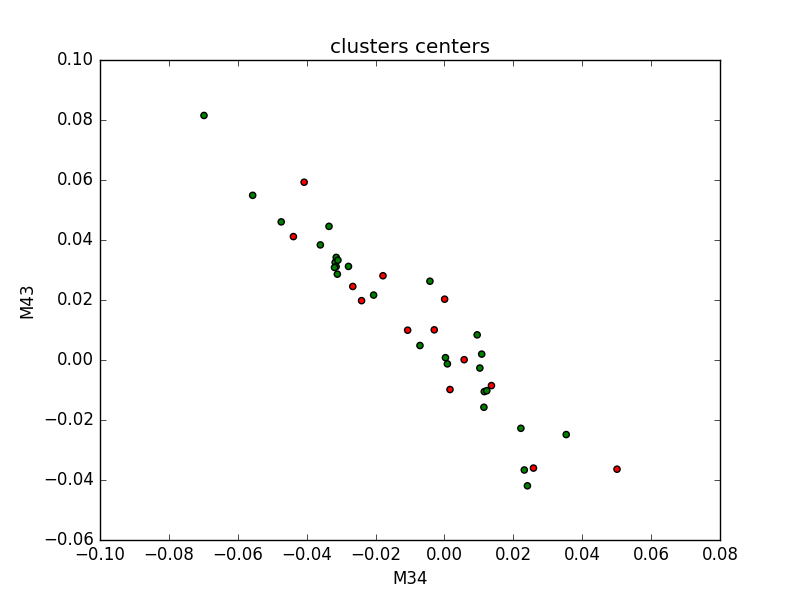
\includegraphics[width=10cm]{PCA_0.png}
\end{figure}
\begin{figure}
  \caption{centre des clusters après transformation}
  \centering
  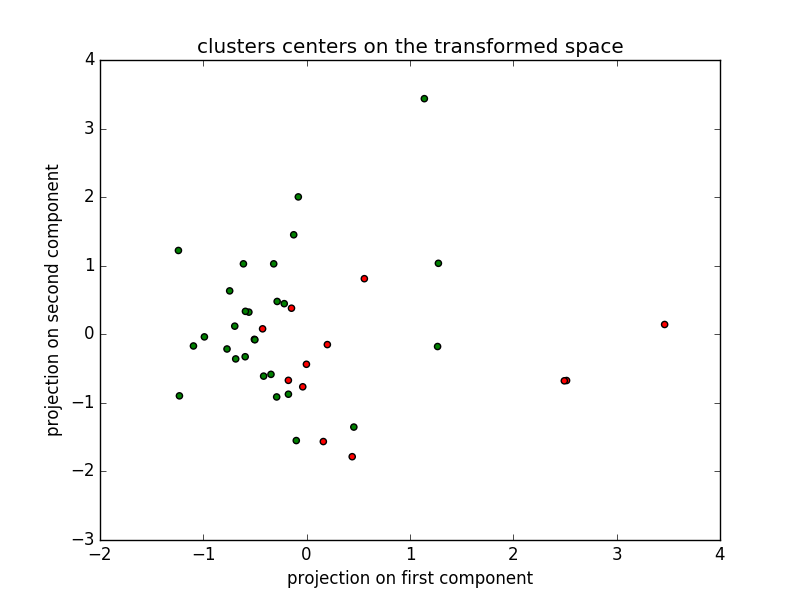
\includegraphics[width=10cm]{PCA_1.png}
\end{figure}
\begin{figure}
  \caption{Part de variance expliquée}
  \centering
  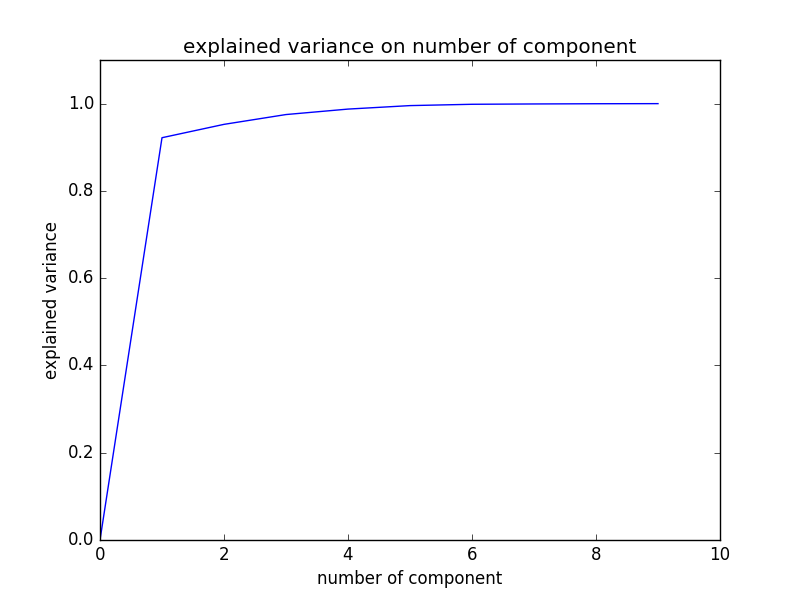
\includegraphics[width=10cm]{PCA_3.png}
\end{figure}
\begin{figure}
  \caption{analyse de la composante principale}
  \centering
  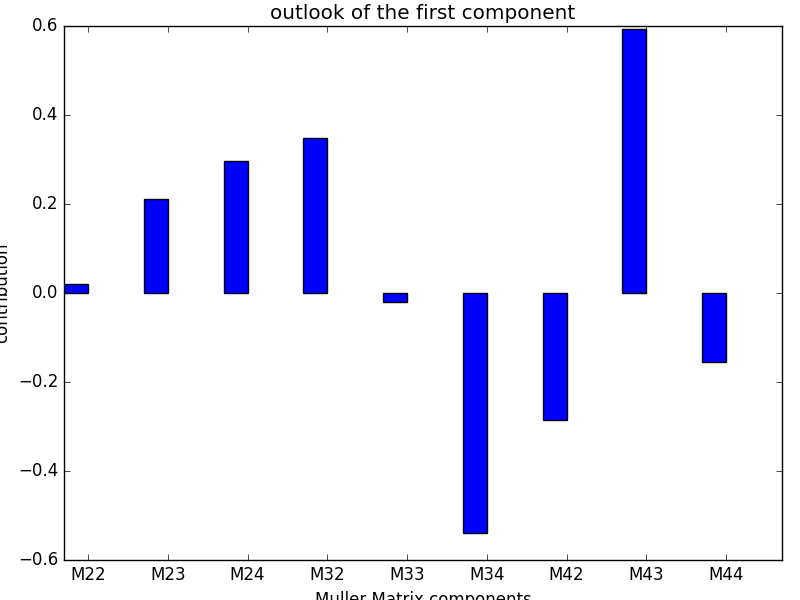
\includegraphics[width=10cm]{PCA_2.png}
\end{figure}

\paragraph{résultats}
La réduction de dimension par PCA semble efficace. La composante principale explique 90\% de la variance (fig 2.3). 
De l'analyse de la première composante (fig 2.4) ressort deux effets principaux :
- La petite contribution des éléments diagonaux de la matrice de Müller
- Le rôle prépondérant de M34 et M43

On remarque une certaine anti-corrélation des éléments de la matrice de Müller. Le poids de M43 est proche de l'opposé de celui de M34. Le poids de M42 est également proche de l'opposé de celui de M24. Cette observation n'est par contre pas vérifiée pour M23 et M32 qui semblent corrélés.
\paragraph{conclusion}
La PCA effectuée sur les centres des clusters valident certaines supposition comme le rôle faible des éléments diagonaux ou le rôle important des éléments M34 et M43.

Par contre, la projection de la PCA en 2 dimensions ne nous permet pas de séparer les données de manière suffisantes pour être capable de distinguer des zones clairement différentes entre les clusters sains et les clusters malades. (fig 2.2)
\section{Méthode de classification}

\subsection{Arbre décisionnel et Random Forest}
\subparagraph{Arbre décisionnel} 
\index{Arbre de décision}
L'arbre décisionnel est une méthode de classification très classique, qui donne souvent de bon résultats. L'idée est trouver un hyperplan qui sépare au mieux les données (parfois très simple, sur une variable uniquement) et de recommencer cela sur les deux sous ensembles de données ainsi crées. On isole ainsi les zones où les points sont similaires, et l'on peut ainsi prédire le diagnostique d'un pixel, les hyperplans permettant de construire un arbre de décision.
\subparagraph{Random Forest}
\index{Arbre de décision}
La Random Forest ou forêt d'arbre, est juste un ensemble d'arbres de décision. Les données sont divisées aléatoirement, puis l'on associe à chaque sous ensemble un arbre de décision. Le résultat de la prédiction se fait par vote, chaque arbre donne sa prédiction, la prédiction majoritaire l'emporte.
\paragraph{Prétraitement utilisé}
Nous avons commencé à apprendre sur toutes les données. Au début nous avions uniquement les pixels, sans les images associés, puis pour préciser les résultats et limiter le sur-apprentissage nous les avons classés par image. Nous avons appris au début sur tous les paramètres de la matrice de Müller, puis uniquement sur les 6 éléments significatifs.
\paragraph{Résultats}
L'apprentissage sur les 16 éléments de la matrice de Müller a résulté dans fort sur-apprentissage : l'arbre de décision réussissait à retrouver l'image de provenance, la forte corrélation entre image et diagnostic ne nous permet donc pas d'aller plus loin. L'apprentissage sur 16 images et le test sur la 17éme a permis de dévoiler ce sur-apprentissage, avec des performances renversées et aléatoires. Sur la figure qui suit on peut voir des résultats très élevés (de l'ordre de 95\%) qui témoignent plus d'un sur-apprentissage que d'un réel résultat. En effet la séparation de par image entre ensemble de test et d'apprentissage donne des résultats beaucoup plus mitigés (autour de 40\%). La restriction à 6 éléments de la matrice n'améliore pas la performance. 
\begin{figure}[htbp]
  \caption{résultats de la Random forest (pixels mélangés)}
  \centering
  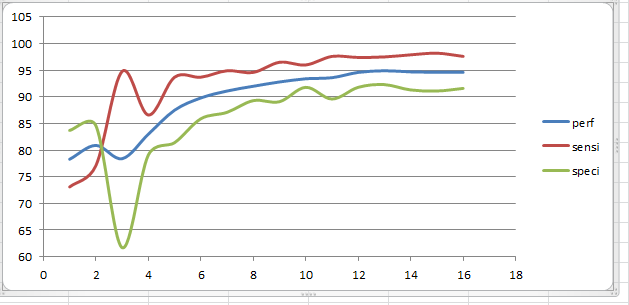
\includegraphics[width=10cm]{RandomForestPerf.png}
\end{figure}
\paragraph{Explication}
Le faible nombre d'images à diagnostic non uniforme conduit l'algorithme à choisir l'image pour déterminer le diagnostic, les différences entre les images étant plus importantes que les différences de diagnostic. L'apprentissage est donc nécessairement biaisé. 
\paragraph{Piste d'amélioration}
Pour résoudre ce problème il faudrait avoir accès à des images au diagnostic varié, images sur lesquelles un réel apprentissage est possible. La difficulté à obtenir ces images nous a poussé a changer de méthode d'apprentissage et à pousser plus loin la compréhension que l'on avait des données.
\subsection{K plus proche voisin}
La méthode des k plus proche voisin consiste à essayer de prédire l’état d'un nouveaux point en se basant sur l'état de ses voisins les plus proches. Cette méthode a l'avantage de pouvoir classer les données selon des schémas non linéaires. Par contre, c'est une méthode sensible à la dimension. 
\paragraph{Prétraitement utilisé}
Nous avons testé la méthodes des KNN sur les centres des clusters pour plusieurs raisons :
- A chaque classification, l'algorithme doit recalculer l'ensemble des distances avec tout l’échantillon d'apprentissage. Il y a donc une nécessité de réduire le nombre de donnée en entrée sur lesquels on calcule les distances.
- De plus, chaque cluster regroupe un ensemble de point très proches les uns des autres. Ainsi, en prenant tous les éléments, les plus proches voisins d'un certain point auraient souvent tous appartenu au même cluster ce qui rend l'information extraite redondante. Cela aurait revenu à utiliser l'algorithme avec 1 seul voisin. 
\paragraph{Résultats}
Les résultats présentés ci dessous corresponde au taux de bonne prédiction en prenant une image de test et en cherchant les k plus proches voisins sur les 16 autres. Chaque cluster est représenté par un vecteur comprenant les éléments suivants de la matrice de Müller : ['M23', 'M24', 'M32', 'M34', 'M42', 'M43'].
\subparagraph{}
\begin{center}
\begin{tabular}{|c|c|}  
  \hline
  échantillon de test & taux de bon résultat \\
  \hline
  1 & 100\%\\
  2 & 0\%\\
  3 & 100\%\\
  4 & 100\%\\
  5 & 0\%\\
  6  & 100\%\\
  7 & 33\%\\  
  8 & 50\%\\
  9 & 66\%\\
  10 & 100\%\\
  11 & 100\%\\
  12 & 100\%\\
  13 & 100\%\\
  14 & 75\%\\
  15 & 66\%\\
  16 & 75\%\\
  17 & 100\%\\
  \hline
  moyenne & 69\%\\  
  \hline
\end{tabular}
\end{center}

En utilisant les 9 éléments de la matrice de Müller Mij avec i et j différents de 1, on obtient un taux moyen de 65%
\paragraph{Conclusion}
Les résultats donnés par les KNN ne sont pas très bon. Piste d'explication?

\subsection{SVM}
\index{SVM}
Les Machines à Vecteurs Support ou SVM (Support Vector Machine) sont des classifieurs qui cherchent à séparer linéairement deux ensembles de points dans un certain espace en maximisant la marge entre ces deux sets de points. Par défault (avec un noyeau linéaire), la séparation est donc nécessairement linéaire. Cependant, en transformant nos données pour les plongées dans un autre espace, souvent de dimension supérieur, on peut générer un modèle de capacité supérieur et fortement non linéaire. C'est ce qu'on appelle le Kernel trick\index{Kernel trick}

\paragraph{Prétraitement utilisé}
Les SVM sont efficaces lorsque le nombre de feature est inférieur (voire très inférieur) au nombre de données. On applique donc cette méthode aux points directement, et non pas aux centres des clusters.

\paragraph{Résultats}

\begin{figure}[H]
  \centering  
  \caption{Résultats de la méthode SVM: proportion de bonnes prédictions et nombre de pixels dans l'ensemble de test, pour chaque image.}
  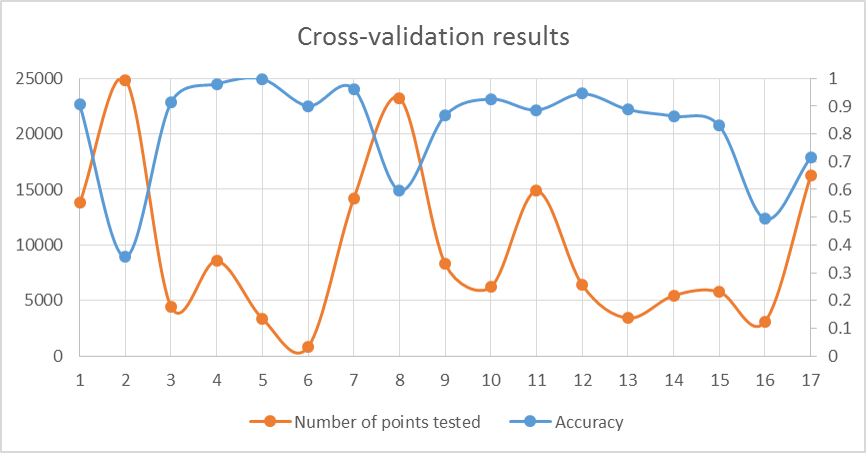
\includegraphics[width=10cm]{SVM_CV.png}
\end{figure}

\paragraph{Explication et Piste d'amélioration}
Le problème du Kernel trick\index{Kernel trick} est qu'il necessitte d'avoir une idée a priori du type de fonction que l'on cherche à estimer pour pouvoir utiliser un noyeau adequat. Ce n'est ici pas le cas, on ne sais pas a priori qu'elle pourrait être le type de fonction permettant de distinguer linéairement un pixel sain d'un pixel malade.

Pour contrer ce problème, il faudrait "apprendre la fonction noyeau". C'est en quelque sorte le rôle des neural networks.\index{Neural networks}. On peut voir les n-1 couches du réseau de neuronnes comme étant la fonction du noyeau et la dernière comme une séparation linéaire sur les données plongées dans ce nouvel espace.

\subsection{Reseaux de Neurones}

Comme évoqué précedemment, les Neural Networks sont une piste naturels à explorer lorsqu'on a pas d'idée a priori de la forme du "bon" noyeau à utiliser dans les SVMs. Un réseau de neuronnes consiste en une succession de couche de neuronnes. La première couche de neuronnes correspond aux données d'entrée et la dernière à la prediction souhaitée. L'avantage principale des réseaux neuronnaux est d'être capable, délors que le réseau a plus de deux couches, d'apprendre des fonctions fortement non linéaires sans apriori sur leur forme. Nous avons utilisé une pénalisation linéaire de la norme des poids. 

\paragraph{prétraitement}
Le prétraitement correspond ici aux choix des données à mettre dans la première couche. Nous avons utilisé un maximum d'input dans un premier temps. Par la suite nous avons pu éstimé le poids final de chacun de  ces inputs pour évaluer quels étaient les inputs important pour la prise de décision. Après plusieurs itérations et tests, nous avons conclus que les éléments les plus importants étaient les suivants :

\begin{itemize}

    \item Les éléments de la matrice de Muller : M32, 	M43, M33, M42

    \item La norme 1 de la matrice de Muller 
    
    \item La norme 2 de la matrice de Muller 

    \item La norme infini de la matrice de Muller  

\end{itemize}

\begin{figure}[htbp]
  \caption{Poids des inputs}
  \centering
  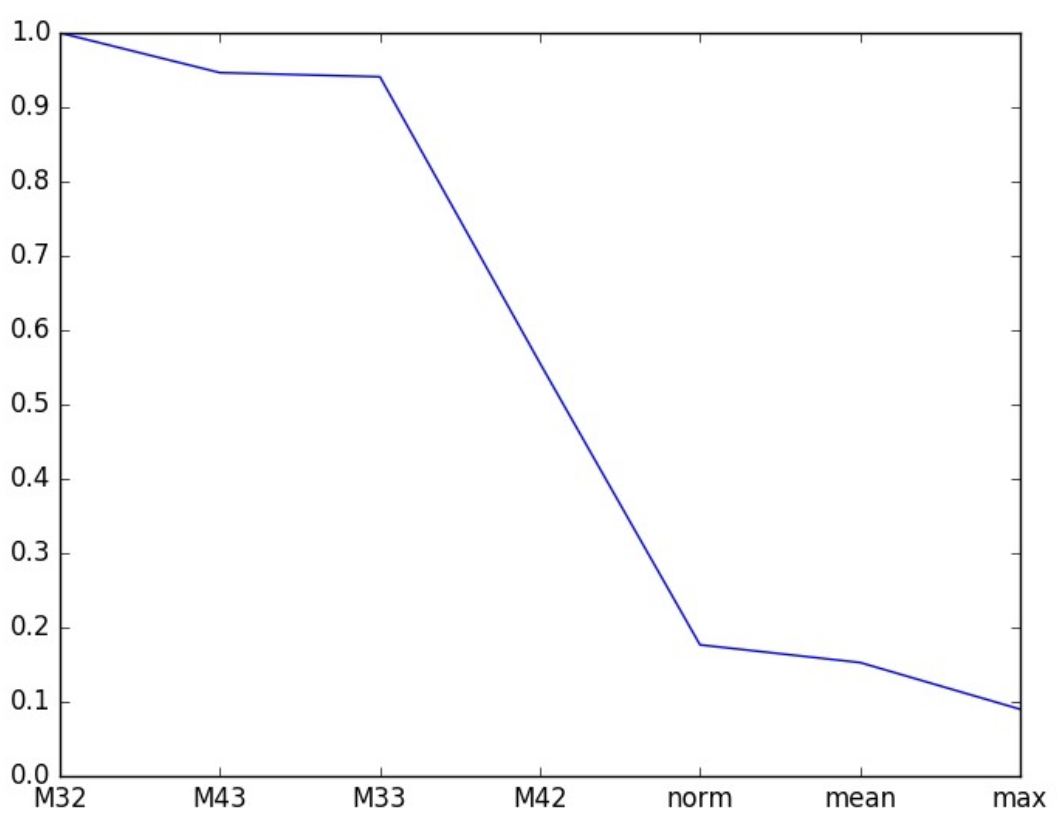
\includegraphics[width=10cm]{input_weight_nn.png}
\end{figure}

\paragraph{Résultats}
Les résultats présentés ici sont obtenus avec un réseaux de quatre couches : [7, 50, 50, 2] et un constante de pénalisation de 0.5.
On obtient un tax de bonnes prédictions moyen de 80\% en effectuant une validation croisée avec un apprentissage sur 16 images et test sur la 17ème. 

Les résultats nous seraient surement améliorés en augmentant le nombre d'itération et en s'appuyant sur un set de donnée plus large. En l'état, les résultas sont comparables à ceux donner par les SVMs.
\begin{figure}[htbp]
  \caption{Résultats de la classification avec des neural networks}
  \centering
  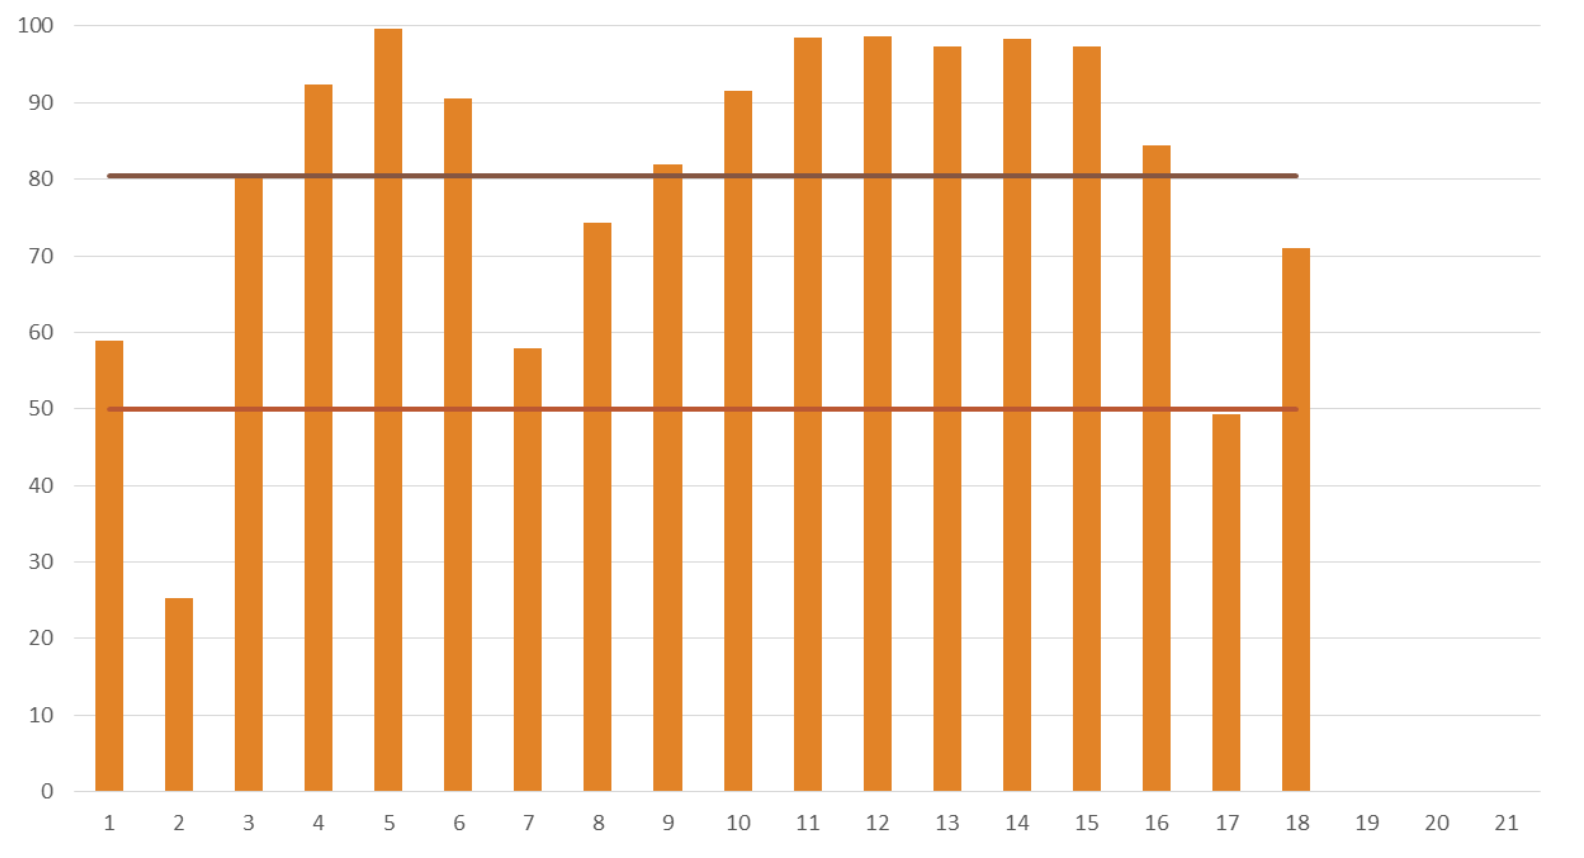
\includegraphics[width=10cm]{nn_results.png}
\end{figure}

\section{Comparaison des méthodes de classifications}

\begin{figure}[htbp]
  \caption{Comparaison des taux de bonne prédiction des différentes méthodes de classification testées.}
  \centering
  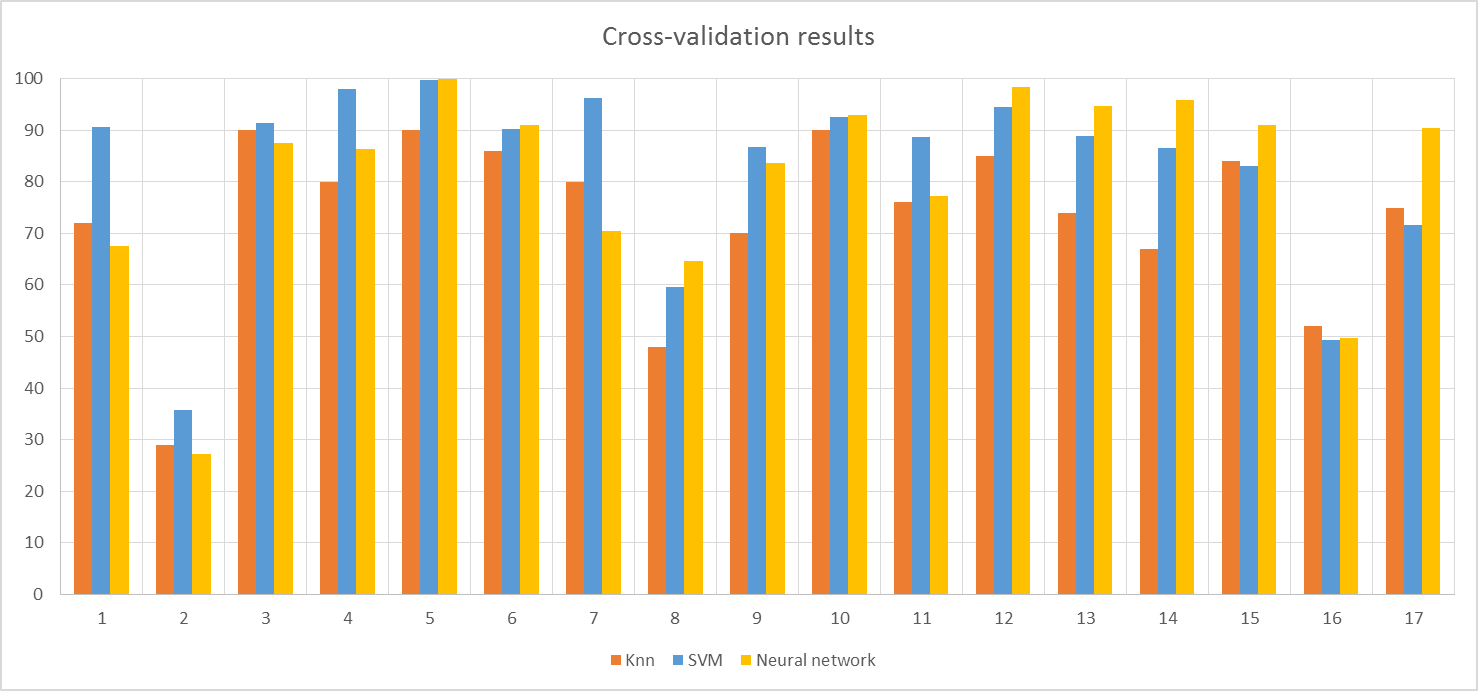
\includegraphics[width=10cm]{Compared_CV.png}
\end{figure}

\begin{center}
Moyenne des taux de précision\\

\begin{tabular}{|c|c|c|}  
  \hline
  Méthode & Moyenne simple & Moyenne pondérée\\
  \hline
  KNN & 73.41 & 65.75\\
  Neural Network & 80.49 & 71.70\\  
  SVM & 82.56 & 75.65\\
  \hline
  Maximum & 85.78 & 79.17\\
  \hline
\end{tabular}
\end{center}

Ce tableau présente les taux de précision moyens des méthodes précédentes, soit en moyennant sur chaque image, soit en pondérant les résultats par le nombre de pixels de l'image (ainsi, chaque pixel intervient 1 fois dans le calcul final, selon sa classification à partir de 16 autres images).
Enfin, on calcule le taux de précision maximal pour les méthodes de classification précédentes, image par image. Si l'on combine les méthodes précédentes, on ne peut pas espérer dépasser cette valeur.


La méthode Knn semble avoir de moins bons résultats que les méthodes SVM et Neural network. 

Par ailleurs, on remarque que les images ayant beaucoup de pixels (les images 2 et 8 représentent 30\% des pixels) ont des moins bons taux de prédiction, ce qui pourrait indiquer que nous n'avons pas atteint le seuil de données critiques nécessaires à des résultats optimaux. Avec quelques images supplémentaires, on pourrait espérer garantir un taux de précision d'au moins 80\% avec cette méthode. 
Notons enfin que l'image 16 a également un taux de précision très faible, en dépit de son petit combre de points. C'est la seule image ayant à la fois des zones saines et malades, il semble donc que les méthodes aient tendance à prédire le même diagnostic pour les pixels d'une même image.
Dans les circonstances actuelles, certaines images ont des résultats très inférieurs à cette valeur moyenne, voire en-deçà de 50\%: ces méthodes ne sont donc pas assez fiable pour permettre de bien classifier les données.

\tableofcontents


\listoffigures
\listoftables
\printindex
\end{document}
